\PassOptionsToPackage{dvipsnames,svgnames,x11names}{xcolor}
\documentclass[tikz,border=8pt]{standalone}
\usetikzlibrary{arrows.meta,positioning,calc,shapes,shadows,decorations.pathmorphing,shapes.geometric,backgrounds,decorations.markings,decorations.pathreplacing,decorations.text,fit,shapes.misc,shapes.arrows,matrix,bending,3d,chains,intersections,shapes.symbols,svg.path,shapes.multipart,snakes,shapes.callouts,angles,quotes}
\providecolor{gold}{RGB}{212,175,55}
\providecolor{silver}{RGB}{192,192,192}
\providecolor{bronze}{RGB}{205,127,50}
\providecolor{darkblue}{RGB}{0,0,139}
\providecolor{lightblue}{RGB}{173,216,230}
\providecolor{darkgreen}{RGB}{0,100,0}
\providecolor{lightgreen}{RGB}{144,238,144}
\providecolor{darkred}{RGB}{139,0,0}
\providecolor{navy}{RGB}{0,0,128}
\providecolor{skyblue}{RGB}{135,206,235}
\providecolor{beige}{RGB}{245,245,220}
\providecolor{cream}{RGB}{255,253,208}
\usepackage{amsmath}
\usepackage{amssymb}
\usepackage{fontawesome5}
\usetikzlibrary{fadings,shadows.blur,patterns,patterns.meta}

\usepackage{xcolor}

% --- COLOR PALETTE ---
\definecolor{svgorange}{RGB}{255, 107, 53}
\definecolor{svggreen}{RGB}{0, 168, 107}
\definecolor{svgblue}{RGB}{41, 128, 185}
\definecolor{viewboxcolor}{HTML}{00A8CC}
\definecolor{viewboxcyan}{HTML}{00E5FF}
\definecolor{gridgray}{RGB}{215, 222, 230}
\definecolor{darktext}{RGB}{44, 62, 80}

\begin{document}
\begin{tikzpicture}[
    % --- STYLES ---
    bubble/.style={
        draw=darktext!25, fill=white, rounded corners=6pt,
        inner sep=10pt, font=\small, text=darktext,
        blur shadow={shadow opacity=20, shadow yshift=-2pt, shadow blur radius=4pt}
    },
    titlebubble/.style={
        draw=none, fill=darktext, rounded corners=8pt,
        text width=14cm, inner sep=12pt, font=\normalfont, text=white,
        blur shadow={shadow opacity=25, shadow yshift=-3pt, shadow blur radius=5pt}
    },
    codebox/.style={
        fill=darktext!6, draw=darktext!20, font=\ttfamily\footnotesize,
        inner sep=4pt, rounded corners=3pt
    },
    arrow/.style={
        -Stealth, thick, color=darktext!80
    }
]

% =========================================================================
% 1. ABSOLUTE WHITE CANVAS BACKGROUND (Layer 1)
% =========================================================================
\fill[white] (-9, 10.5) rectangle (19, -16);

% =========================================================================
% 2. INFINITE GRID (Layer 2)
% =========================================================================
\draw[step=0.2cm, gridgray!35, very thin] (-8, 10) grid (18, -15);
\draw[step=1cm, gridgray!70, thin] (-8, 10) grid (18, -15);

% =========================================================================
% 3. VECTOR SHAPES (Layer 3)
% =========================================================================
% Path P1: Spans outside the viewBox domain
\draw[line width=4pt, svgorange, line cap=round]
    (-2, 2) .. controls (1, 4) and (2, -2) .. (5, -5) .. controls (2, -8) and (12, -8) .. (13, -2);

% Polygon G1: Fully contained inside the viewBox
\filldraw[top color=svgblue!35, bottom color=svgblue!75, draw=svgblue, line width=2pt, rounded corners=1pt]
    (2, -2) -- (3, -4) -- (5, -3) -- (4, -1) -- cycle;

% Circle C1: Partially overlapping the viewBox boundary at (10, -10)
\filldraw[top color=svggreen!25, bottom color=svggreen!65, draw=svggreen, line width=2pt]
    (10, -10) circle (3cm);

% =========================================================================
% 4. CLIPPING MASK (Layer 4)
% =========================================================================
% Outside region is dimmed (opacity 0.85), inside viewBox is 100% transparent
\fill[white, fill opacity=0.85, even odd rule]
    (-9, 10.5) rectangle (19, -16)
    (0, 0) rectangle (10, -10);

% =========================================================================
% 5. INFINITE AXES (Layer 5)
% =========================================================================
% X Axis (Positive Right)
\draw[-Stealth=3.5mm, very thick, darktext] (-8, 0) -- (18, 0);
\node[right, font=\bfseries, text=darktext] at (18.2, 0) {X-Axis ($\infty$)};

% Y Axis (Positive Downward in SVG Specification) - Truncated to avoid Title Bubble collision
\draw[-Stealth=3.5mm, very thick, darktext] (0, 6.5) -- (0, -15);
\node[below, font=\bfseries, text=darktext] at (0, -15.5) {Y-Axis ($\infty$, Positive Down)};

% Origin Node & Label
\node[circle, fill=darktext, inner sep=2.5pt] at (0, 0) {};
\node[font=\footnotesize\bfseries, color=darktext, anchor=east] at (-1.8708,0.1217) {(0,0) Origin};

% =========================================================================
% 6. VIEWBOX DASHED BORDER (Layer 6)
% =========================================================================
\draw[preaction={draw, white, line width=4pt}, line width=2.5pt, dashed, viewboxcolor] (0, 0) rectangle (10, -10);

% =========================================================================
% 7. VIEWBOX DIMENSIONS AND TICKS (Layer 7)
% =========================================================================
% Width Dimension Indicator & Label (Elevated above shapes)
\draw[Stealth-Stealth, thick, viewboxcolor] (0, 2.5) -- (10, 2.5);
\node[font=\bfseries, text=viewboxcolor, anchor=south] at (5, 2.8) {width: "100"};

% Height Dimension Indicator & Label (Text shifted left)
\draw[Stealth-Stealth, thick, viewboxcolor] (-1.5, 0) -- (-1.5, -10);
\node[font=\bfseries, text=viewboxcolor, anchor=south, rotate=90] at (-2.5, -5) {height: "100"};

% Internal origin coordinate offsets
\node[font=\bfseries\footnotesize, text=viewboxcolor, anchor=west] at (0.5, -0.5) {min-x: 0};
\node[font=\bfseries\footnotesize, text=viewboxcolor, anchor=west] at (0.5, -1.0) {min-y: 0};

% Numerical Scale Mapping Ticks
\draw[thick, darktext] (5, 0.2) -- (5, -0.2);
\node[font=\scriptsize\bfseries, fill=white, inner sep=1pt] at (5, 0.6) {SVG $x=50$};

\draw[thick, darktext] (10, 0.2) -- (10, -0.2);
\node[font=\scriptsize\bfseries, fill=white, inner sep=1pt] at (10, -0.6) {SVG $x=100$};

\draw[thick, darktext] (0.2, -10) -- (-0.2, -10);
\node[font=\scriptsize\bfseries, fill=white, inner sep=1pt, anchor=east] at (-2.5, -10) {SVG $y=100$};

% =========================================================================
% 8. SHAPE LABELS & SAFE POINTERS (Layer 8)
% =========================================================================
% P1 Label & Arrow (Shifted to clear path)
\node[font=\footnotesize\bfseries, color=svgorange, fill=white, fill opacity=1, text opacity=1, inner sep=3pt, rounded corners=2pt, draw=svgorange!30, blur shadow={shadow opacity=15, shadow yshift=-1pt, shadow blur radius=2pt}] at (-6.0, 2.0) {Path $P_1$ (Out of bounds)};
\draw[arrow, color=svgorange] (-4.1647,2) -- (-2.2, 2.2);

% G1 Label & Arrow
\node[font=\footnotesize\bfseries, color=svgblue, fill=white, fill opacity=1, text opacity=1, inner sep=3pt, rounded corners=2pt, draw=svgblue!30, blur shadow={shadow opacity=15, shadow yshift=-1pt, shadow blur radius=2pt}] at (4.5, -4.5) {Polygon $G_1$};
\draw[arrow, color=svgblue] (4, -4.5) -- (4, -3.5);

% C1 Label & Arrow
\node[font=\footnotesize\bfseries, color=svggreen!90!black, fill=white, fill opacity=1, text opacity=1, inner sep=3pt, rounded corners=2pt, draw=svggreen!30, blur shadow={shadow opacity=15, shadow yshift=-1pt, shadow blur radius=2pt}] at (10, -14.5) {Circle $C_1$};
\draw[arrow, color=svggreen] (10, -14) -- (10, -13);

% =========================================================================
% 9. COMPLEX ANNOTATIONS & POINTERS (Layer 9)
% =========================================================================
% Annotation A: Endless Space (Nudged to align with P1 label)
\node[bubble, text width=4.5cm] (annoA) at (-5.5, 6.5) {
    \textbf{\color{darktext}\faInfinity \quad Endless Coordinate Space}\\[2pt]
    Coordinates like \texttt{x="150"} or \texttt{x="-50"} are perfectly valid. The path data mathematically exists here regardless of whether it is visible on the screen.
};
\fill[darktext] (-2, 6.5) circle (1.5pt);
\node[above, font=\tiny\bfseries, text=darktext] at (-2, 6.6) {SVG (-20, -65)};
\draw[arrow] (-2.9323,6.5176) -- (-2.1, 6.5);

% Annotation B: The viewBox Attribute
\node[bubble, text width=5.5cm] (annoB) at (15, 4) {
    \textbf{\color{viewboxcolor}\faCrop \quad The viewBox Attribute}\\[2pt]
    \tikz\node[codebox]{<svg viewBox="0 0 100 100">};\\
    This dictates: "Start at origin $(0,0)$, and frame a window $100$ units wide and $100$ units tall." This establishes the \textit{local fractional aspect ratio} (1:1 in this case).
};
\draw[arrow, color=viewboxcolor] (11.9676,2.9413) -- (8, 0);

% Annotation C: Visual Clipping
\node[bubble, text width=5.5cm] (annoC) at (16, -13) {
    \textbf{\color{svggreen}\faCut \quad Visual Clipping}\\[2pt]
    Elements intersecting the \texttt{viewBox} perimeter (like this circle at $x=100, y=100$) are clipped by the DOM's rendering engine. Only the segment inside the $0-100$ domain is passed to the CSS scaling engine.
};
\draw[arrow, color=svggreen] (12.9933,-13) -- (12.12, -12.12);

% =========================================================================
% 10. TITLE BUBBLE (Layer 10)
% =========================================================================
\node[titlebubble] at (5.5738,9.274) {
    {\Large\bfseries \faVectorSquare \quad The SVG Infinite Plane \& The viewBox Lens}\\[4pt]
    \normalsize In SVG, vector data exists on a boundless Cartesian plane (where $+Y$ goes down). The \texttt{viewBox} attribute defines a specific fractional mathematical region to be extracted and projected into the HTML DOM. Anything outside this bounding box is conceptually clipped or ignored during responsive mapping.
};

\end{tikzpicture}
\end{document}
